\documentclass[conference]{IEEEtran}
\usepackage[utf8]{inputenc}
\usepackage[T1]{fontenc}
\usepackage[french]{babel}
\usepackage{cite}
\usepackage{amsmath,amssymb}
\usepackage{graphicx}
\usepackage{booktabs}
\usepackage{array}
\usepackage{url}
\usepackage[hidelinks]{hyperref}
\graphicspath{{resultats/figures/}{../resultats/figures/}}

\hyphenation{By-zan-tine Ten-der-mint qua-rum}

\begin{document}

\renewcommand{\abstractname}{Résumé}
\renewcommand{\IEEEkeywordsname}{Mots-clés}

\title{Consensus BFT pour un consortium universitaire :\\
sécurité, cohérence et performances entre universités de l'UEMOA}

\author{%
\IEEEauthorblockN{Souleymane Kone, Mouhamadou Makhtar Gueye et Fatou Kine Thioub}
\IEEEauthorblockA{École Supérieure Polytechnique, Université Cheikh Anta Diop\\
Laboratoire LITA, Dakar, Sénégal\\
Groupe 3 --- module Cryptographie \& Technologies Blockchain}
}

\maketitle

\begin{abstract}
Les universités de l'UEMOA doivent vérifier des diplômes délivrés par d'autres établissements, souvent dans un autre pays. Une base centrale réduirait les délais, mais créerait un point unique de défaillance et de confiance. Cet article étudie un registre répliqué entre universités, où chaque établissement exploite un validateur CometBFT et où l'empreinte des diplômes est inscrite par consensus. La question est de savoir dans quelle mesure un consensus BFT garantit la sécurité et la cohérence des transactions tout en maintenant des performances acceptables. Nous combinons une analyse des quorums et des phases de PBFT avec un banc d'essai CometBFT v0.38.17 à 4, 7 et 10 validateurs, des retards réseau de 10 à 45 ms, puis des arrêts de validateurs sur la configuration à 4. Les mesures montrent une latence moyenne de 1\,303 ms sans retard, de 1\,365 ms avec retard et de 1\,401 à 1\,403 ms à 7 et 10 validateurs, pour un débit de 14,1 à 15,3 tx/s. Avec un validateur arrêté, la latence moyenne monte à 2\,258 ms, le p95 à 5\,698 ms et le débit tombe à 5,9 tx/s. Avec deux validateurs arrêtés sur quatre, la chaîne se bloque sans diverger. La cohérence tient donc sous $f$ pannes, mais la vivacité est le point faible ; la tolérance à un validateur qui ment reste une garantie théorique, non provoquée dans notre banc.
\end{abstract}

\begin{IEEEkeywords}
consensus BFT, PBFT, CometBFT, blockchain de consortium, UEMOA, tolérance aux fautes byzantines, diplômes, performance.
\end{IEEEkeywords}

\section{Introduction}

\IEEEPARstart{L}{a} vérification d'un diplôme est un acte de confiance. Un employeur, une administration ou une autre université doit s'assurer qu'un document a bien été délivré par l'établissement qu'il mentionne, à la date indiquée, pour la formation annoncée. Dans l'Union économique et monétaire ouest-africaine (UEMOA), cette vérification se heurte à trois difficultés : la distance entre établissements, l'hétérogénéité des procédures et la circulation de documents falsifiés. La presse sénégalaise en fait régulièrement état, mais ces sources restent journalistiques et doivent être recoupées avec des données officielles \cite{dakaractu2025,ndarinfo2026}.

Une première réponse consiste à centraliser les diplômes dans une base nationale ou régionale. La vérification devient rapide, mais un tel système crée un point unique de défaillance, un administrateur unique et une confiance institutionnelle forte. Une seconde réponse consiste à répartir le registre entre les universités : chaque établissement conserve une copie, les inscriptions sont répliquées et les vérificateurs comparent l'empreinte d'un diplôme à celle du registre. C'est le schéma d'une \emph{blockchain de consortium} : un réseau fermé, où l'identité des participants est connue et où l'on n'ouvre pas la participation à n'importe qui \cite{androulaki2018fabric,wust2018blockchain}.

Le verrou technique est le consensus. Dans un consortium, une université peut tomber en panne, mais elle peut aussi se comporter mal : envoyer des messages contradictoires, voter deux fois, ou tenter de faire croire à deux historiques différents. Un protocole qui ne tolère que les pannes franches, comme Raft ou PBFT dans sa version crash, ne suffit pas si l'on veut se prémunir contre un participant malveillant. Les protocoles \emph{Byzantine fault-tolerant} (BFT) tolèrent jusqu'à $f$ validateurs fautifs parmi $n$, à condition que $n \geq 3f+1$ \cite{lamport1982byzantine,castro1999pbft}. Cette garantie a un coût : davantage de messages, des quorums plus larges, des changements de vue et une sensibilité accrue aux délais réseau.

La question de recherche de cet article est la suivante : \emph{dans quelle mesure un protocole de consensus BFT garantit-il la sécurité et la cohérence des transactions tout en maintenant des performances acceptables dans un consortium universitaire soumis à des comportements byzantins ?} Nous faisons l'hypothèse que la cohérence tient tant que moins d'un tiers des validateurs est fautif, mais que les performances se dégradent avec le nombre de validateurs et les perturbations réseau. Nous distinguons trois notions souvent confondues : la \emph{sûreté} (deux validateurs honnêtes ne décident pas de valeurs contradictoires), la \emph{vivacité} (le système finit par décider) et la \emph{véracité} (la valeur décidée est correcte). Un consensus BFT garantit les deux premières sous ses hypothèses ; il ne garantit pas la troisième. Un diplôme faux peut être inscrit si l'université émettrice le déclare valide.

Nos contributions sont les suivantes.

\begin{enumerate}
\item Nous explicitons le lien entre seuil de tolérance, taille de quorum et intersection des quorums, et nous montrons pourquoi $n \geq 3f+1$ est la condition structurante.
\item Nous construisons un banc d'essai CometBFT reproductible à 4, 7 et 10 validateurs, avec des retards réseau injectés, puis des arrêts de validateurs sur la configuration à 4, et nous publions les mesures brutes, les scripts et les figures.
\item Nous montrons que, dans notre banc, le passage de 4 à 10 validateurs coûte peu en latence et en débit, alors que l'arrêt de $f+1$ validateurs bloque la chaîne ; le facteur dominant est donc la disponibilité d'un quorum, pas la croissance quadratique des messages à cette échelle.
\item Nous discutons les limites de l'expérience, en particulier l'absence de faute byzantine active, et nous en tirons des recommandations pour un déploiement progressif.
\end{enumerate}

Le reste de l'article est organisé comme suit. La section~\ref{sec:contexte} présente le contexte et la question. La section~\ref{sec:etat} situe le travail dans l'état de l'art. La section~\ref{sec:fondements} rappelle les fondements du consensus BFT. La section~\ref{sec:methode} décrit le banc d'essai. La section~\ref{sec:resultats} présente les résultats. La section~\ref{sec:discussion} discute les implications et les menaces à la validité. La section~\ref{sec:conclusion} conclut.

\section{Contexte et question de recherche}
\label{sec:contexte}

\subsection{Le problème des diplômes dans l'UEMOA}

Les universités de l'espace UEMOA délivrent des diplômes qui circulent au-delà des frontières. Un étudiant formé à Dakar peut candidater à Ouagadougou, à Abidjan ou à Lomé ; un employeur peut demander une vérification à distance. Les procédures actuelles reposent souvent sur un courrier, un courriel, un cachet ou un appel téléphonique. Elles sont lentes, coûteuses et dépendantes de la disponibilité du service émetteur. La falsification de diplômes est un risque documenté par la presse, mais l'ampleur exacte du phénomène reste mal mesurée \cite{dakaractu2025,ndarinfo2026}.

Le paiement mobile montre que la région sait adopter des infrastructures numériques à grande échelle : la BCEAO recense 60,6 millions de comptes de monnaie électronique actifs fin 2025 et 160\,415 milliards de FCFA échangés en 2024 \cite{bceao2025}. Ce n'est pas un argument technique, mais un argument de contexte : les usagers et les institutions sont déjà habitués à des services numériques interopérables. Un registre de diplômes pourrait s'appuyer sur cette culture numérique, à condition de résoudre la gouvernance et la confiance.

\subsection{Pourquoi un registre répliqué ?}

Une base centrale est simple à concevoir, mais elle concentre les risques. Si le serveur tombe, la vérification s'arrête ; si l'administrateur est compromis, l'historique peut être réécrit ; si un pays héberge la base, les autres pays dépendent de lui. Un registre répliqué entre universités réduit le point unique de défaillance : chaque établissement détient une copie, et les décisions sont prises par un quorum. La contrepartie est la complexité du consensus et la nécessité d'un modèle de faute adapté.

Le cas d'usage est volontairement restreint. Il ne s'agit pas de mettre tout le dossier académique sur une blockchain, ni de remplacer les diplômes papier. Il s'agit d'inscrire une \emph{empreinte} : un identifiant de diplôme, une fonction de hachage du document, l'établissement émetteur, la date et un statut. Les données personnelles restent hors chaîne ; le registre ne contient qu'une preuve d'existence et d'intégrité. Cette séparation réduit les risques de confidentialité et le volume de données.

\subsection{Question et hypothèse}

La question est celle de la section précédente. Nous la décomposons en trois sous-questions :

\begin{enumerate}
\item \textbf{Sûreté :} deux validateurs honnêtes peuvent-ils décider de blocs contradictoires à la même hauteur ?
\item \textbf{Vivacité :} combien de validateurs peuvent être indisponibles avant que la chaîne cesse de progresser ?
\item \textbf{Performance :} comment la latence et le débit évoluent-ils avec le nombre de validateurs et les pannes ?
\end{enumerate}

L'hypothèse est que la sûreté tient sous $f$ fautes, que la vivacité tient tant que $n-p \geq 2f+1$ ($p$ étant le nombre de validateurs indisponibles), et que la performance se dégrade modérément avec $n$ mais fortement avec les pannes. Le critère de réfutation de la partie performance est le suivant : si, à configuration égale, la latence ne change pas significativement entre 4 et 10 validateurs, alors l'hypothèse d'une dégradation avec $n$ est fausse à cette échelle. Nous verrons que c'est partiellement le cas.

\section{État de l'art}
\label{sec:etat}

\subsection{Du problème des généraux byzantins aux quorums}

Lamport, Shostak et Pease formalisent en 1982 le problème des généraux byzantins : des généraux doivent s'accorder sur une décision alors que certains peuvent trahir et envoyer des messages contradictoires \cite{lamport1982byzantine}. Ils montrent qu'un accord déterministe à messages oraux exige $n \geq 3f+1$ et que les signatures permettent de réduire le nombre de messages sans supprimer le seuil. Cette borne est le point de départ de tous les protocoles BFT pratiques.

Fischer, Lynch et Paterson montrent en 1985 qu'aucun protocole déterministe ne peut garantir l'accord dans un réseau asynchrone avec ne serait-ce qu'un processus fautif \cite{fischer1985flp}. Ce résultat, connu sous le nom de FLP, ne condamne pas les blockchains : il indique qu'il faut une hypothèse de synchronisation partielle, ou un protocole probabiliste, pour garantir la vivacité. Les protocoles BFT modernes supposent qu'après un instant inconnu appelé \emph{Global Stabilization Time} (GST), les messages arrivent en temps borné. La sûreté, elle, ne dépend pas de cette borne.

\subsection{PBFT}

Castro et Liskov publient PBFT en 1999 \cite{castro1999pbft}. Le protocole organise un consensus en vues : un primaire propose, les répliques préparent, puis confirment. Une décision est prise lorsqu'un quorum de $2f+1$ répliques a confirmé. Le coût est en $O(n^2)$ messages par décision, ce qui limite pratiquement $n$ à quelques dizaines de validateurs. PBFT introduit aussi les changements de vue : si le primaire est fautif ou trop lent, les répliques élisent un nouveau primaire. La sûreté repose sur l'intersection des quorums et sur les verrous : une réplique honnête ne vote pas pour deux blocs incompatibles à la même hauteur.

\subsection{Tendermint et CometBFT}

Tendermint, dont CometBFT est l'implémentation actuelle, adapte les idées de PBFT à un contexte de blockchain \cite{buchman2018tendermint,cometbft2024}. Le consensus procède par hauteurs et par tours. Un proposer diffuse un bloc ; les validateurs diffusent un \emph{prevote} ; si un quorum de $2f+1$ prevotes est atteint, ils diffusent un \emph{precommit} ; si un quorum de $2f+1$ precommits est atteint, le bloc est décidé. Le bloc suivant peut alors commencer. La finalité est immédiate : une fois décidé, un bloc n'est pas réorganisé, contrairement aux blockchains à preuve de travail.

CometBFT sépare le moteur de consensus de l'application via une interface appelée ABCI. L'application peut être un \texttt{kvstore}, un contrat ou un registre de diplômes. Cette séparation est importante pour notre cas : le consensus ne connaît pas la sémantique des diplômes ; il ordonne des transactions. La validité métier doit être vérifiée par l'application.

\subsection{HotStuff et les protocoles à changement de vue linéaire}

HotStuff réduit le coût des changements de vue à $O(n)$ et introduit une pipeline de phases \cite{yin2019hotstuff}. Il est à la base de plusieurs systèmes de consortium et de blockchains récentes. Son intérêt pour un consortium universitaire est la réduction du coût de communication lorsque le primaire change souvent. En contrepartie, la simplicité de PBFT et la maturité de CometBFT restent des arguments forts pour un déploiement pédagogique et progressif.

\subsection{Blockchains de consortium et évaluation}

Hyperledger Fabric est l'exemple le plus étudié de blockchain permissionnée \cite{androulaki2018fabric}. Il sépare l'exécution, l'ordonnancement et la validation, et propose plusieurs ordonnanceurs, dont des bibliothèques BFT \cite{barger2021bft}. BLOCKBENCH propose une méthodologie d'évaluation des blockchains privées, avec des métriques de débit, de latence et de scalabilité \cite{dinh2017blockbench}. Notre travail s'inscrit dans cette lignée, mais à une échelle volontairement réduite : un consortium de 4 à 10 universités, un registre de diplômes, et une question de faisabilité plutôt qu'un classement de plateformes.

\subsection{Ce qui manque}

La littérature compare souvent les plateformes à grande échelle, avec des charges de travail de type bancaire ou IoT. Peu de travaux étudient un consortium universitaire de petite taille, avec des latences ouest-africaines et une question de gouvernance explicite. Notre apport n'est pas un nouveau protocole, mais une étude de cas reproductible : nous mesurons CometBFT dans une configuration réaliste pour un consortium, nous distinguons les pannes des fautes byzantines, et nous publions les données et le code.

\section{Fondements du consensus BFT}
\label{sec:fondements}

\subsection{Modèle de système et de faute}

Nous considérons $n$ validateurs, dont au plus $f$ sont fautifs. Un validateur honnête suit le protocole ; un validateur fautif peut envoyer des messages arbitraires, omettre des messages, ou envoyer des messages différents à des destinataires différents. Les canaux sont authentifiés : un message forgé par un adversaire ne peut pas se faire passer pour un honnête. Le réseau est partiellement synchrone : après GST, tout message entre honnêtes arrive en temps borné ; avant GST, il peut être arbitrairement retardé.

Ce modèle est plus fort que le modèle crash, où un nœud fautif s'arrête simplement. C'est aussi plus réaliste pour un consortium : une université peut être compromise, un administrateur peut vouloir favoriser un diplôme, ou un serveur peut envoyer des messages incohérents à cause d'un bug. La contrepartie est un coût plus élevé : $n \geq 3f+1$ au lieu de $n \geq 2f+1$ pour les protocoles crash.

\subsection{Quorums et intersection}

Un quorum est un sous-ensemble de validateurs de taille $q = 2f+1$. Deux quorums quelconques se recoupent sur au moins
\begin{equation}
|Q_1 \cap Q_2| \geq 2q - n = 2(2f+1) - (3f+1) = f+1
\end{equation}
validateurs. Comme au plus $f$ validateurs sont fautifs, l'intersection contient au moins un honnête. C'est cette intersection qui empêche deux décisions contradictoires : un honnête ne peut pas voter pour deux valeurs incompatibles à la même hauteur. La figure~\ref{fig:quorums}(a) illustre le cas $n=4$, $f=1$ : deux quorums de 3 se recoupent sur 2 nœuds, dont au moins un honnête.

\begin{figure*}[t]
\centering
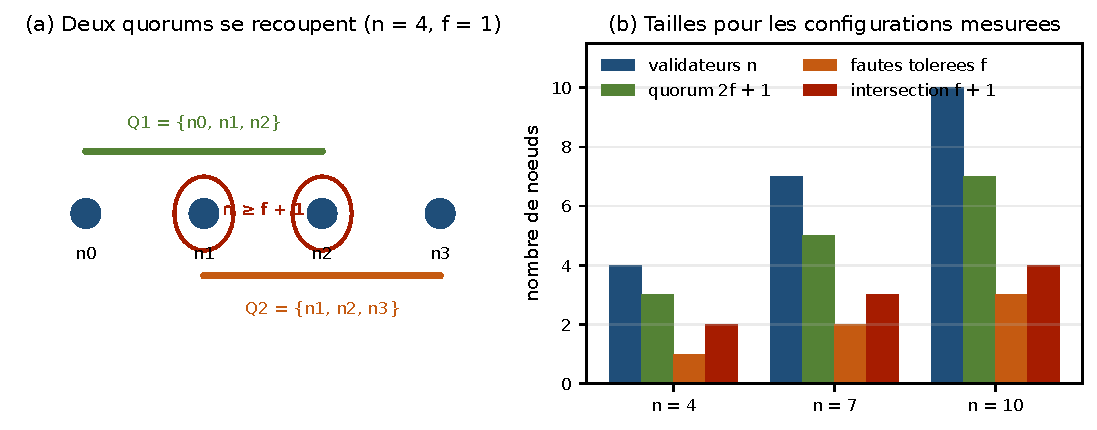
\includegraphics[width=0.92\textwidth]{fig1_quorums.pdf}
\caption{(a) Deux quorums de taille $2f+1$ dans un consortium de $n=4$ validateurs se recoupent sur au moins $f+1=2$ nœuds. (b) Tailles pour les configurations mesurées : $n=4,7,10$, $f=1,2,3$, quorum $3,5,7$.}
\label{fig:quorums}
\end{figure*}

La figure~\ref{fig:quorums}(b) donne les valeurs pour nos configurations. Pour $n=4$, $f=1$, le quorum est 3 ; pour $n=7$, $f=2$, le quorum est 5 ; pour $n=10$, $f=3$, le quorum est 7. On voit que le nombre de fautes tolérées augmente lentement : il faut passer de 4 à 7 validateurs pour tolérer une faute de plus, et de 7 à 10 pour en tolérer une troisième. C'est le prix de la tolérance byzantine.

\subsection{Phases et coût de PBFT}

La figure~\ref{fig:phases} présente une séquence simplifiée de PBFT. Le client envoie une requête au primaire. Le primaire diffuse un \emph{pre-prepare} contenant le numéro de vue, le numéro de séquence et le bloc. Chaque réplique qui accepte le pre-prepare diffuse un \emph{prepare} à tous. Lorsqu'une réplique a reçu $2f$ messages prepare compatibles (plus le sien), elle diffuse un \emph{commit}. Lorsqu'elle a reçu $2f+1$ commits, elle exécute et répond au client. Le client attend $f+1$ réponses identiques pour accepter le résultat.

\begin{figure*}[t]
\centering
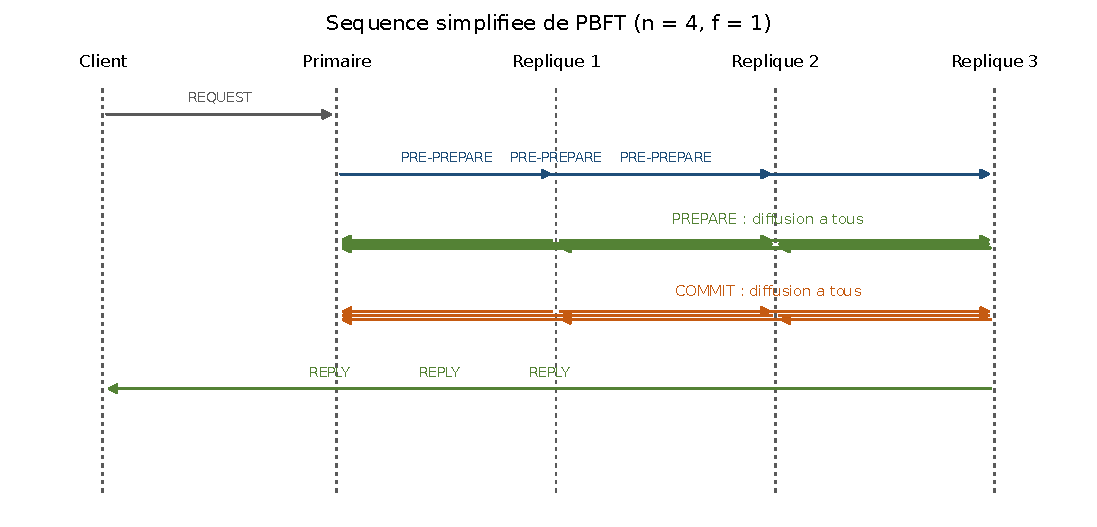
\includegraphics[width=0.88\textwidth]{fig2_phases_pbft.pdf}
\caption{Séquence simplifiée de PBFT pour $n=4$, $f=1$. Les phases prepare et commit sont des diffusions à tous ; le coût total est en $O(n^2)$ messages par décision.}
\label{fig:phases}
\end{figure*}

Le nombre de messages par décision, en comptant la requête, le pre-prepare, les prepare, les commit et les réponses, est
\begin{equation}
1 + (n-1) + (n-1)^2 + n(n-1) + n = 2n^2 - n.
\end{equation}
Pour $n=4$, on obtient 28 messages ; pour $n=7$, 91 ; pour $n=10$, 190. La croissance est quadratique, ce qui explique pourquoi PBFT est adapté à un petit consortium et non à des milliers de validateurs. La figure~\ref{fig:messages} illustre cette croissance.

\begin{figure}[t]
\centering
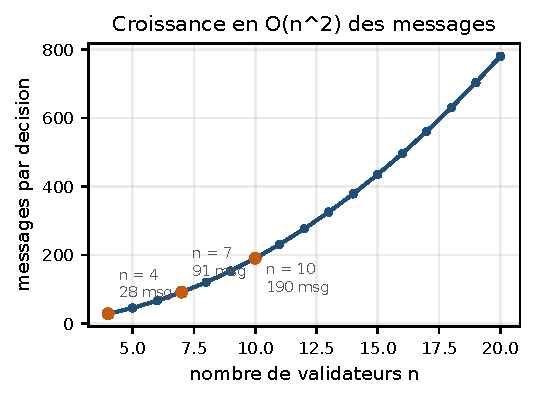
\includegraphics[width=\columnwidth]{fig6_messages.pdf}
\caption{Nombre de messages par décision dans PBFT, $2n^2-n$. Les points marquent les configurations mesurées : 28, 91 et 190 messages pour $n=4,7,10$.}
\label{fig:messages}
\end{figure}

\subsection{Sûreté et vivacité}

La sûreté se démontre par l'absurde. Supposons que deux validateurs honnêtes décident deux blocs différents à la même hauteur. Chaque décision exige un quorum de $2f+1$ validateurs. Les deux quorums se recoupent sur au moins $f+1$ validateurs, dont au moins un est honnête. Cet honnête aurait voté pour deux blocs incompatibles, ce qui contredit le protocole. La sûreté ne dépend donc pas de la synchronisation : elle tient même si le réseau est arbitrairement lent.

La vivacité est plus fragile. Elle exige qu'après GST, un proposer honnête puisse faire circuler son bloc et qu'un quorum de $2f+1$ validateurs honnêtes soit disponible. Si plus de $f$ validateurs sont indisponibles, il peut rester moins de $2f+1$ validateurs honnêtes, et aucun quorum ne peut se former. Le système peut aussi être bloqué par un primaire fautif, mais un changement de vue doit alors permettre d'élire un nouveau primaire. C'est pourquoi les protocoles BFT utilisent des timeouts et des changements de vue : la vivacité est garantie \emph{après GST}, pas avant.

\subsection{CometBFT en pratique}

CometBFT implémente un consensus de type Tendermint, avec des hauteurs et des tours. Le moteur propose un bloc, collecte les prevotes, puis les precommits. Le paramètre \texttt{timeout\_commit} introduit un délai entre la fin d'un bloc et le début du suivant ; dans notre configuration, il vaut 1 s. C'est une source de latence incompressible qui explique pourquoi nos mesures sont supérieures à la seconde même sur un réseau local. Le paramètre \texttt{create\_empty\_blocks\_interval} vaut 0 s : CometBFT crée des blocs vides pour maintenir la progression, ce qui permet de mesurer la hauteur même sans transaction.

Cette architecture a une conséquence pour notre cas d'usage : le débit utile peut être faible, mais la chaîne continue de produire des blocs. Pour un registre de diplômes, c'est acceptable : les inscriptions sont rares par rapport aux blocs, et la finalité rapide importe plus que le débit brut.

\section{Méthode et banc d'essai}
\label{sec:methode}

\subsection{Plateforme et topologie}

Nous utilisons CometBFT v0.38.17, l'application \texttt{kvstore} fournie avec le moteur, et Docker. Chaque validateur est un conteneur qui exécute \texttt{cometbft node}. Le réseau de test est généré par \texttt{cometbft testnet}, puis les configurations sont ajustées : \texttt{addr\_book\_strict = false} et \texttt{allow\_duplicate\_ip = true} pour permettre à plusieurs conteneurs de cohabiter sur la même machine. Les clés de validation sont générées localement et ne sont pas publiées.

Les expériences ont été réalisées sur une machine à 8 cœurs et 10 Go de mémoire. Les validateurs partagent le même processeur, ce qui limite la portée des résultats : nous mesurons un comportement fonctionnel et une latence de consensus, pas une performance de production. La topologie est un réseau Docker bridge ; les conteneurs se joignent par leur nom d'hôte.

\begin{table}[t]
\caption{Retards aller simple injectés avec \texttt{tc netem}. Les villes sont fictives ; les valeurs sont des ordres de grandeur, pas des mesures de terrain.}
\label{tab:latences}
\centering
\footnotesize
\begin{tabular}{@{}llr@{}}
\toprule
Nœud & Ville (université fictive) & Retard \\
\midrule
node0 & Dakar (UCAD) & 10 ms \\
node1 & Saint-Louis (UGB) & 15 ms \\
node2 & Ouagadougou (Ki-Zerbo) & 40 ms \\
node3 & Abidjan (Houphouët-Boigny) & 35 ms \\
node4 & Bamako & 40 ms \\
node5 & Niamey & 45 ms \\
node6 & Lomé & 35 ms \\
node7 & Cotonou & 35 ms \\
node8 & Bissau & 20 ms \\
node9 & Ziguinchor & 15 ms \\
\bottomrule
\end{tabular}
\end{table}

Le tableau~\ref{tab:latences} donne les retards injectés. Ils sont appliqués avec \texttt{tc qdisc replace dev eth0 root netem delay Xms 5ms}. La gigue de 5 ms ajoute une variabilité contrôlée. Ces valeurs ne prétendent pas représenter la latence réelle entre capitales : elles servent à tester la sensibilité du consensus à des délais de quelques dizaines de millisecondes. Une mesure de terrain devrait utiliser une matrice de latences entre universités, par exemple avec des sondes RIPE Atlas ou des mesures \texttt{ping} répétées.

\subsection{Scénarios et charge}

Quatre scénarios sont définis.

\begin{itemize}
\item \textbf{S1} : 4 validateurs, sans retard ajouté. C'est la référence locale.
\item \textbf{S2} : 4 validateurs, avec les retards du tableau~\ref{tab:latences}.
\item \textbf{S3} : 7 puis 10 validateurs, avec retards.
\item \textbf{S4} : 4 validateurs, arrêt de $f=1$ puis de $f+1=2$ validateurs, puis redémarrage.
\end{itemize}

Pour chaque scénario opérationnel, nous effectuons trois essais indépendants. Chaque essai comprend 20 transactions séquentielles pour la latence, puis 200 transactions avec 20 envois simultanés pour le débit. Les transactions sont des chaînes de la forme \texttt{diplome-<identifiant>=valide}, sans donnée personnelle. Le client mesure le temps de \texttt{broadcast\_tx\_commit}, qui inclut la diffusion, le consensus et le retour du nœud. Le p95 est calculé sur les latences triées.

Pour S4, nous utilisons 50 transactions pour le scénario avec $f=1$ panne, et 10 transactions pour le scénario avec $f+1$ pannes. Nous suivons la hauteur de bloc toutes les 0,5 s pendant l'arrêt et la reprise, ce qui produit la chronologie de la figure~\ref{fig:pannes}. Le temps de reprise est mesuré entre le redémarrage des conteneurs et l'apparition du premier nouveau bloc. Les p95 reposent sur 20 mesures (10 seulement pour S4) : ils donnent un ordre de grandeur de la queue de latence, pas une estimation stable.

\subsection{Métriques et traitement statistique}

Les métriques sont la latence moyenne, la médiane, le p95, le débit, le nombre de transactions validées et la hauteur de bloc. Pour agréger trois essais, nous utilisons la moyenne, l'écart-type d'échantillon et un intervalle de confiance à 95 \% avec $t=4{,}303$ pour deux degrés de liberté. Les intervalles sont larges, car nous n'avons que trois essais ; ils servent à éviter de surinterpréter des écarts de quelques millisecondes.

Le débit est calculé comme le nombre de transactions validées divisé par la durée totale des envois. Il est borné par le client, qui utilise 20 fils d'exécution. Il ne représente donc pas la capacité maximale de CometBFT, mais un débit applicatif réaliste pour un petit consortium.

\subsection{Reproductibilité et éthique}

Tous les scripts sont dans \texttt{code/}. \texttt{code/reproduire.sh} régénère les figures et les tableaux à partir des données de \texttt{resultats/}. \texttt{code/experimenter.sh} reconstruit un réseau de test et rejoue les scénarios ; il faut Docker et environ 8 Go de mémoire. Les clés de validation ne sont jamais publiées, et le dossier \texttt{testnet/} est exclu du dépôt. Aucun système réel n'est attaqué : le banc est local, les universités sont fictives et les diplômes sont synthétiques. L'usage d'un outil d'IA générative pour l'aide à la rédaction et à la mise en forme est déclaré.

\section{Résultats}
\label{sec:resultats}

\subsection{Latence et débit}

Le tableau~\ref{tab:resultats} résume les mesures. Sans retard (S1), la latence moyenne est de 1\,303 ms avec un intervalle de confiance de $\pm 9$ ms, et le débit de 15,3 tx/s. Avec les retards UEMOA (S2), la latence passe à 1\,365 ms ($\pm 27$ ms) et le débit à 14,6 tx/s. Le passage de 4 à 7 validateurs (S3) donne 1\,403 ms ($\pm 29$ ms) et 14,1 tx/s ; le passage à 10 validateurs donne 1\,401 ms ($\pm 16$ ms) et 14,1 tx/s.

\begin{table*}[t]
\caption{Résultats agrégés sur trois essais par scénario (moyenne $\pm$ écart-type ; IC95 pour la latence). Le scénario S4 à $f+1$ pannes est bloqué.}
\label{tab:resultats}
\centering
\footnotesize
\begin{tabular}{@{}lcccccc@{}}
\toprule
Scénario & $n$ & Pannes & Latence moyenne & IC95 & p95 & Débit \\
\midrule
S1 : référence, sans retard & 4 & 0 & 1\,303 ms $\pm$ 4 ms & $\pm$ 9 ms & 1\,317 ms & 15,3 tx/s \\
S2 : retard UEMOA & 4 & 0 & 1\,365 ms $\pm$ 11 ms & $\pm$ 27 ms & 1\,417 ms & 14,6 tx/s \\
S3 : sept validateurs & 7 & 0 & 1\,403 ms $\pm$ 12 ms & $\pm$ 29 ms & 1\,503 ms & 14,1 tx/s \\
S3 : dix validateurs & 10 & 0 & 1\,401 ms $\pm$ 7 ms & $\pm$ 16 ms & 1\,526 ms & 14,1 tx/s \\
S4 : $f=1$ panne & 4 & 1 & 2\,258 ms $\pm$ 91 ms & $\pm$ 227 ms & 5\,698 ms & 5,9 tx/s \\
S4 : $f+1=2$ pannes & 4 & 2 & bloqué & --- & --- & 0 tx/s \\
\bottomrule
\end{tabular}
\end{table*}

La figure~\ref{fig:latence}(a) montre les moyennes et les écarts-types ; la figure~\ref{fig:latence}(b) montre les p95. La latence de S1 est dominée par le \texttt{timeout\_commit} de 1 s : le consensus lui-même est plus rapide, mais le moteur attend avant de commencer le bloc suivant. C'est une décision de configuration, pas une limite fondamentale. Avec un timeout plus court, la latence baisserait, au prix d'un risque accru de changements de vue sur un réseau lent.

\begin{figure*}[t]
\centering
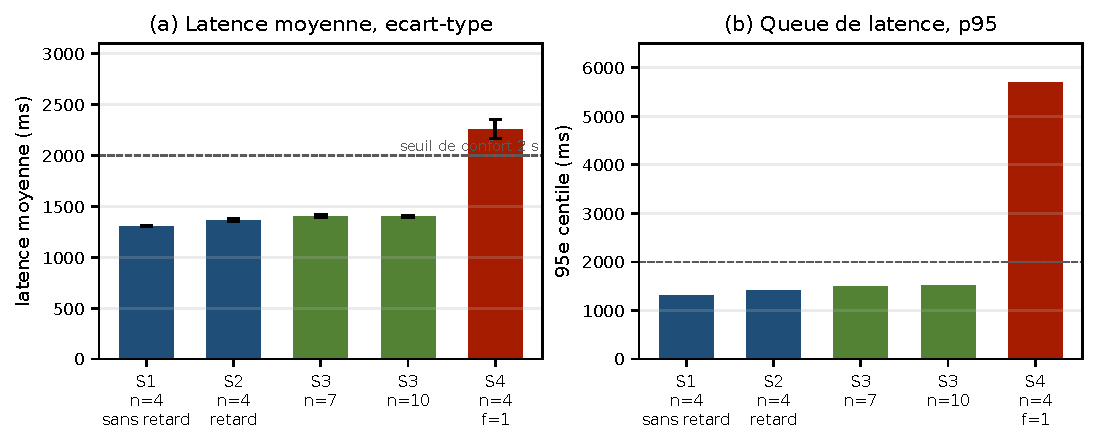
\includegraphics[width=0.95\textwidth]{fig3_latence.pdf}
\caption{Latence par scénario. (a) Moyenne et écart-type. (b) 95\textsuperscript{e} centile. Le seuil de 2 s est un repère de confort pour une vérification interactive ; il n'a pas de valeur normative.}
\label{fig:latence}
\end{figure*}

Le débit (figure~\ref{fig:debit}) baisse de 15,3 à 14,6 tx/s avec le retard, puis à 14,1 tx/s à 7 et 10 validateurs. La baisse entre S1 et S3 est d'environ 7,8 \%, ce qui est modeste. En revanche, avec $f=1$ panne, le débit tombe à 5,9 tx/s, soit une division par 2,6. Avec $f+1=2$ pannes, le débit est nul : la chaîne est bloquée.

\begin{figure}[t]
\centering
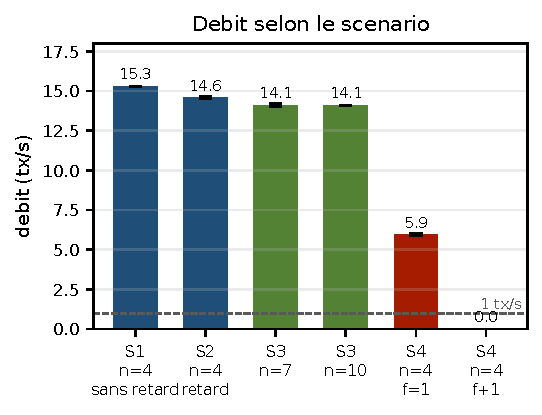
\includegraphics[width=\columnwidth]{fig4_debit.pdf}
\caption{Débit par scénario. Le scénario $f+1$ est hachuré : la chaîne est bloquée et aucune transaction n'est validée.}
\label{fig:debit}
\end{figure}

\subsection{Effet du nombre de validateurs}

Contrairement à l'hypothèse naïve d'une dégradation forte avec $n$, nous n'observons pas de différence significative entre 7 et 10 validateurs : 1\,403 ms contre 1\,401 ms, avec des intervalles qui se recoupent largement. Le débit est identique (14,1 tx/s). Cela ne contredit pas la théorie : le coût en messages augmente, mais à cette échelle, il n'est pas le facteur limitant. Le \texttt{timeout\_commit}, la latence réseau et le client de mesure dominent. Le passage de 4 à 7 validateurs ajoute environ 39 ms de latence moyenne, ce qui reste modeste.

Ce résultat est important pour un consortium universitaire : il n'est pas nécessaire de limiter le nombre d'universités à 4 pour des raisons de performance. En revanche, chaque université supplémentaire augmente le coût de gouvernance, le nombre de clés à gérer et la complexité des accords. La limite pratique vient moins du consensus que de l'organisation.

\subsection{Pannes et reprise}

La figure~\ref{fig:pannes} montre la chronologie réelle. Pendant la phase nominale, la hauteur augmente régulièrement. Lorsque nous arrêtons un validateur ($f=1$), la chaîne continue : il reste 3 validateurs sur 4, soit exactement le quorum de 3. La hauteur avance, mais plus lentement, et les transactions peuvent subir des timeouts. La moyenne monte à 2\,258 ms, la médiane reste autour de 1,4 s, mais le p95 atteint 5\,698 ms : la queue de latence explose, pas la médiane.

Lorsque nous arrêtons un second validateur ($f+1=2$), il ne reste que 2 validateurs sur 4, en dessous du quorum de 3. La hauteur reste constante, les transactions échouent, et la chaîne se bloque. Aucune bifurcation n'est observée : la sûreté tient, la vivacité non. C'est exactement le comportement attendu du modèle : $n-p \geq 2f+1$ devient $4-2=2 < 3$.

\begin{figure*}[t]
\centering
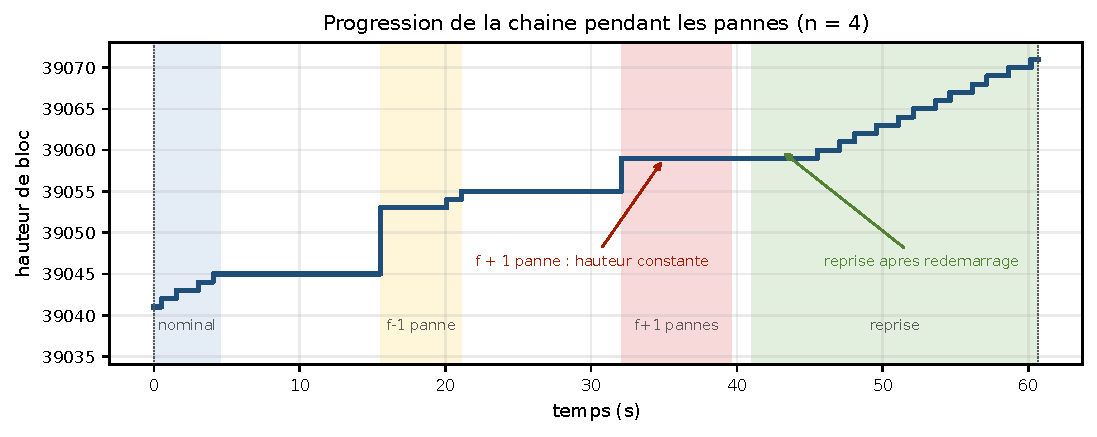
\includegraphics[width=0.95\textwidth]{fig5_pannes.pdf}
\caption{Chronologie réelle de la hauteur de bloc pendant l'arrêt de validateurs et la reprise ($n=4$). Avec $f=1$ panne, la chaîne continue ; avec $f+1=2$ pannes, elle se bloque sans diverger.}
\label{fig:pannes}
\end{figure*}

Après redémarrage des deux validateurs, le premier nouveau bloc apparaît après 8,6 s. La chaîne reprend à la hauteur suivante, sans rollback visible. Ce délai inclut le temps de démarrage des conteneurs, la reconnexion au réseau et le prochain tour de consensus. Il serait plus court avec des validateurs déjà démarrés et un réseau stable, mais il donne un ordre de grandeur pour la reprise après incident.

\subsection{Coût en messages}

Le tableau~\ref{tab:messages} et la figure~\ref{fig:messages} donnent le nombre de messages par décision. Pour $n=4$, 28 messages ; pour $n=7$, 91 ; pour $n=10$, 190. Le passage de 4 à 10 multiplie le coût par 6,8. Dans notre banc, cette croissance ne se traduit pas par une baisse proportionnelle du débit, car le temps de consensus n'est pas dominé par les messages. À plus grande échelle, ou avec des liens réseau plus lents, le coût en messages deviendrait limitant.

\begin{table}[t]
\caption{Coût théorique en messages par décision et quorum pour les configurations mesurées.}
\label{tab:messages}
\centering
\footnotesize
\begin{tabular}{@{}rrrr@{}}
\toprule
$n$ & $f$ & Quorum $2f+1$ & Messages $2n^2-n$ \\
\midrule
4 & 1 & 3 & 28 \\
7 & 2 & 5 & 91 \\
10 & 3 & 7 & 190 \\
\bottomrule
\end{tabular}
\end{table}

\subsection{Synthèse des résultats}

Trois enseignements se dégagent. Premièrement, la latence reste de l'ordre de 1,3 à 1,5 s pour 4 à 10 validateurs, ce qui est compatible avec une vérification de diplôme. Deuxièmement, la panne d'un validateur dégrade surtout la queue de latence et le débit, pas la médiane : le système reste utilisable, mais moins prévisible. Troisièmement, la panne de $f+1$ validateurs bloque la chaîne sans divergence : la sûreté est robuste, la vivacité est le point faible.

\section{Discussion}
\label{sec:discussion}

\subsection{Réponse à la question de recherche}

La question demandait dans quelle mesure un consensus BFT garantit la sécurité et la cohérence tout en maintenant des performances acceptables. La réponse est nuancée. La \emph{cohérence} est garantie par le protocole tant que $n \geq 3f+1$ et que les validateurs honnêtes suivent les règles : nos mesures ne montrent aucune divergence, même lorsque la chaîne se bloque. La \emph{sécurité} au sens de la sûreté tient donc sous les hypothèses du modèle. En revanche, la \emph{vivacité} n'est pas garantie dès que $f+1$ validateurs sont indisponibles, et la \emph{véracité} des diplômes n'est pas garantie du tout : le consensus ordonne ce que les universités lui donnent.

Les performances sont acceptables pour le cas d'usage : une latence de 1,3 à 1,5 s et un débit de 14 à 15 tx/s suffisent pour inscrire et vérifier des diplômes, dont le volume est faible par rapport à celui des paiements. La dégradation en panne reste tolérable pour $f$ pannes, mais la queue p95 à 5,7 s peut être gênante pour une vérification interactive. La panne de $f+1$ validateurs est un arrêt de service, pas une corruption : c'est un risque opérationnel qu'il faut anticiper par la redondance et la surveillance.

\subsection{BFT ou CFT ?}

Si le seul risque est la panne franche, un protocole CFT comme Raft serait plus simple et plus rapide. Mais un consortium universitaire n'est pas un centre de données unique : les établissements ont des intérêts distincts, des administrations distinctes et des niveaux de sécurité hétérogènes. Un validateur compromis peut vouloir favoriser un diplôme ou bloquer un concurrent. Le modèle BFT est donc justifié par la menace, pas par la mode. Le coût supplémentaire est le prix de cette hypothèse.

Il faut toutefois être honnête : notre banc ne teste que des pannes franches. La tolérance byzantine est argumentée par la théorie et par l'intersection des quorums, mais elle n'est pas provoquée expérimentalement. Un test complet demanderait un validateur byzantin qui double vote, envoie des messages contradictoires ou refuse de répondre de façon sélective. C'est la principale limite de notre travail.

\subsection{Gouvernance et véracité}

Le consensus ne dit pas si un diplôme est vrai. Il dit que les universités s'accordent sur l'ordre des inscriptions. Si une université émettrice inscrit un faux diplôme, le consensus le validera. La véracité dépend donc de la vérification métier : signature de l'établissement, contrôle de l'identité de l'étudiant, règles d'accréditation. Le registre apporte une preuve d'intégrité et d'antériorité, pas une preuve de vérité.

La gouvernance est l'autre moitié du problème. Qui admet une nouvelle université ? Qui révoque une clé compromise ? Que faire d'un diplôme dont l'émetteur conteste l'inscription ? Comment traiter un établissement qui quitte le consortium ? Ces questions ne se résolvent pas dans le code ; elles demandent un règlement, un comité et des procédures. Un consortium de 4 à 7 universités est plus facile à gouverner qu'un consortium de 10, même si les performances techniques ne se dégradent pas.

\subsection{Confidentialité et données personnelles}

Le registre ne contient que des empreintes et des métadonnées. Les données personnelles restent hors chaîne. Cette séparation réduit les risques, mais elle ne les supprime pas : une empreinte de diplôme peut être corrélée à une personne si l'espace des diplômes est petit. Il faut donc saler les empreintes, limiter l'accès aux métadonnées et prévoir un droit à l'effacement pour les données hors chaîne. La conformité avec les règles de protection des données doit être étudiée avant le déploiement.

\subsection{Coût et soutenabilité}

Un consortium permissionné n'utilise pas de preuve de travail : l'énergie consommée est celle de quelques serveurs, pas d'un réseau mondial de mineurs. Le coût principal est humain et organisationnel : administration des clés, surveillance, audits, formation. Pour des universités aux budgets contraints, ce coût doit être mutualisé. Une infrastructure régionale partagée, avec des validateurs hébergés par chaque université, est plus réaliste qu'un déploiement isolé par établissement.

\subsection{Menaces à la validité}

\textbf{Validité interne.} Les validateurs partagent une machine, ce qui favorise les communications et limite les effets de la charge. Le client de mesure utilise 20 fils, ce qui borne le débit. Le \texttt{timeout\_commit} de 1 s domine la latence. Les pannes sont des arrêts de conteneur, pas des fautes byzantines. Les résultats doivent donc être lus comme une étude de faisabilité, pas comme un benchmark de production.

\textbf{Validité externe.} Les latences sont des ordres de grandeur, pas une matrice mesurée entre capitales. Les universités sont fictives. Le nombre de validateurs (4 à 10) est petit. Un déploiement réel aurait des liens plus hétérogènes, des pannes plus variées et des attaques plus complexes.

\textbf{Validité de construit.} La latence mesurée inclut le \texttt{timeout\_commit} et le client, pas seulement le consensus. Le débit mesure une charge applicative, pas la capacité maximale. Le nombre de messages est un calcul analytique, pas une mesure réseau.

\textbf{Validité de conclusion.} Nous concluons sur la sûreté et la vivacité à partir de la théorie et de pannes franches. La tolérance byzantine active reste une hypothèse, non un résultat expérimental. Les recommandations de gouvernance sont qualitatives.

\subsection{Recommandations}

Pour un consortium universitaire de l'UEMOA, nous recommandons :

\begin{enumerate}
\item \textbf{Commencer petit} : 4 à 7 validateurs, avec un validateur par université et des observateurs non validateurs.
\item \textbf{Prévoir $f=1$ panne} : dimensionner le quorum pour tolérer au moins un validateur indisponible, et surveiller le nombre de validateurs actifs.
\item \textbf{Tester les pannes} : organiser des exercices de coupure et mesurer le temps de reprise, comme dans la figure~\ref{fig:pannes}.
\item \textbf{Traiter la gouvernance} : règlement d'admission, révocation des clés, gestion des litiges, procédure de sortie.
\item \textbf{Ne pas confondre registre et vérité} : conserver la vérification métier et la signature de l'établissement émetteur.
\item \textbf{Prévoir la migration cryptographique} : les signatures du consensus devront peut-être évoluer vers des schémas post-quantiques ; la gouvernance des clés doit permettre cette transition.
\end{enumerate}

\section{Conclusion}
\label{sec:conclusion}

Cet article a étudié un consortium universitaire de l'UEMOA qui utilise un consensus BFT pour inscrire et vérifier des diplômes. Nous avons combiné une analyse des quorums et des phases de PBFT avec un banc d'essai CometBFT à 4, 7 et 10 validateurs, des retards réseau injectés et des arrêts de validateurs. Les résultats montrent une latence de 1,3 à 1,5 s et un débit de 14 à 15 tx/s pour 4 à 10 validateurs, avec une dégradation modérée lorsque le nombre de validateurs augmente. Avec $f=1$ panne, la latence moyenne monte à 2,3 s et le débit tombe à 5,9 tx/s ; avec $f+1=2$ pannes, la chaîne se bloque sans diverger. La cohérence tient donc sous $f$ pannes, mais la vivacité est le point faible, et la tolérance à un validateur qui ment reste une garantie théorique dans notre banc.

La réponse à la question de recherche est donc conditionnelle : un consensus BFT garantit la sécurité et la cohérence \emph{si} les hypothèses de faute et de quorum sont respectées, et il offre des performances acceptables pour un registre de diplômes \emph{si} l'on accepte une latence de l'ordre de la seconde et un débit modeste. Il ne garantit ni la disponibilité au-delà de $f$ pannes, ni la véracité des diplômes, ni la gouvernance du consortium. Ces trois dimensions doivent être traitées par l'organisation, pas par le protocole.

Les perspectives sont expérimentales et organisationnelles. Sur le plan expérimental, il faut tester un validateur byzantin actif, mesurer une matrice de latences réelles entre universités, et comparer CometBFT à HotStuff et à Hyperledger Fabric sur le même cas d'usage. Sur le plan organisationnel, il faut définir le règlement du consortium, la gestion des clés, la procédure de révocation et le cadre juridique de la vérification. C'est à ce prix qu'un registre répliqué deviendra une infrastructure utile, et non une démonstration technique.

\section*{Remerciements}

Les auteurs remercient le Pr Gervais Mendy pour le cadrage du module, les groupes 2 et 7 pour les échanges sur les sujets A14 et A1, et les discutants du groupe 7 pour leurs questions. Les mesures ont été réalisées sur le banc de test du groupe 3.

\section*{Déclaration d'usage de l'IA}

Un outil d'IA générative a été utilisé pour aider à structurer le dépôt, à mettre en forme le LaTeX et à relire le français. Les mesures, les choix de protocole, les sources et l'interprétation ont été vérifiés par les trois auteurs.

\bibliographystyle{IEEEtran}
\IfFileExists{../bibliographie/references.bib}{%
  \bibliography{../bibliographie/references}}{%
  \bibliography{bibliographie/references}}

\end{document}
